\documentclass{article}

%Packages
%	Front
\usepackage[T1]{fontenc}
\usepackage[utf8]{inputenc}
%	From template
\usepackage{tabularx}
\usepackage{booktabs}
%	Mine
\usepackage{cite}
\usepackage{graphicx}
\usepackage{indentfirst}
\usepackage{amsmath}
\usepackage{cleveref}
\usepackage{float}

\title{CAS 741: Problem Statement\\STEM Moir{\'e} GPA}

\author{Alexandre Pofelski \\
macid: pofelska}

\date{15 September 2017}

%% Comments

\usepackage{color}

\newif\ifcomments\commentstrue

\ifcomments
\newcommand{\authornote}[3]{\textcolor{#1}{[#3 ---#2]}}
\newcommand{\todo}[1]{\textcolor{red}{[TODO: #1]}}
\else
\newcommand{\authornote}[3]{}
\newcommand{\todo}[1]{}
\fi

\newcommand{\wss}[1]{\authornote{blue}{SS}{#1}}
\newcommand{\an}[1]{\authornote{magenta}{Author}{#1}}



\begin{document}

\maketitle
\clearpage

\begin{table}[hp]
\caption{Revision History} \label{TblRevisionHistory}
\begin{tabularx}{\textwidth}{llX}
\toprule
\textbf{Date} & \textbf{Developer(s)} & \textbf{Change}\\
\midrule
15/09/2017 & Alex & First draft\\
\bottomrule
\end{tabularx}
\end{table}

\clearpage
\tableofcontents
\clearpage

\section{Introduction}
The success of semiconductor devices application in the past decades couldn't have been possible without developing methods able to characterize them. Build and interconnect billions of transistors with each other on a cm$^{2}$ chip is a real challenge such as measuring the gate length of one of them. Scanning Transmission Electron Microscopy (STEM) revealed to be a particularly adapted characterization method in order to probe matter at atomic scale. Nowadays, with aberration correctors, it is possible without much difficulty to form a small electron probe capable to resolve a spacing down to 50pm. Such probe is smaller than the atomic spacing by an order of magnitude therefore, by scanning the probe on the sample and collecting the electrons that crossed it from separate locations (pixels) to form an electron micrograph, it is possible to image the atomic arrangement of matter. The scanning range can be extended to a few microns making STEM an efficient technique to characterize a classic semiconductor device nowadays present in any smartphones.\par \medskip
Variety of parameters are affecting the performance of a semiconductor device at a transistor level. Temperature, defect density, doping concentration are few examples known to influence the transistor behaviour. Some secondary parameters like the elastic deformation is also affecting the device performance by changing the mobility of carriers within the semiconductor material. In current technologies the silicon underneath the gate of a transistor (channel) must be elastically deformed to reach the level of performance desired by the market. Methods to measure locally and quantitatively the elastic strain in crystals were thus massively developed in the last decades in order to help the design of such strained semiconductor devices. One method called Geometric Phase Analysis (GPA) emerged above its competitor because of its easiness and elegance in quantifying strain from an atomically resolved STEM electron micrograph (or image). The Fourier based processing method enabled GPA to isolate and track quantitatively the aperiodicities in the image to convert them into relative strain fields \cite{Hytch1998}. A sensitivity down to $10^-3$ is claimed by the STEM GPA method with a resolution of roughly 1nm. \par \medskip
Nevertheless, the STEM GPA technique is relatively limited in how spatially extended a strain map can be. Since a minimum of a few pixels are needed to image the atomic spacing, the number of pixels of the detection system is limiting the field of view (FOV) of the electron micrograph. With 16 millions pixels a FOV up to 150nm can be reached. The more pixels are used the greater is the FOV however with more pixels, the processing is more demanding. To overcome this issue, a technique based on Moir{\'e} interferometry has been recently developed. The method reveals to be capable of reaching a few microns of FOV while keeping the applicability of the GPA method. The principle is to make interfere the scanning grid of the STEM probe with the crystalline lattice of matter by choosing a scanning step close but not equal to the atomic spacing (undersampling condition). The resulting interference generates a STEM Moir{\'e}hologram displaying an altered version of the sample structural properties on a larger FOV at a cost of a poorer resolution compared to the STEM GPA. In order to be treatable by the GPA method, the hologram needs to be converted by removing the artefact generated by the sampling condition chosen \cite{Pofelski2017}. The STEM Moire GPA method enables thus the strain field from larger devices to be characterized up to a few microns.

\section{Objective}

As a scientific program developer, the objective is to implement a program capable of converting a STEM Moir{\'e} hologram into quantitative relative strain maps. The relative strain maps correspond to two dimensional (2D) maps from the 3 components of the 2D strain tensor and a 2D map of the 2D rotation tensor component. The expectations of the program are summarized in \cref{fig:STEM_Moire_GPA_Objective}

\begin{figure}[H]
\centering
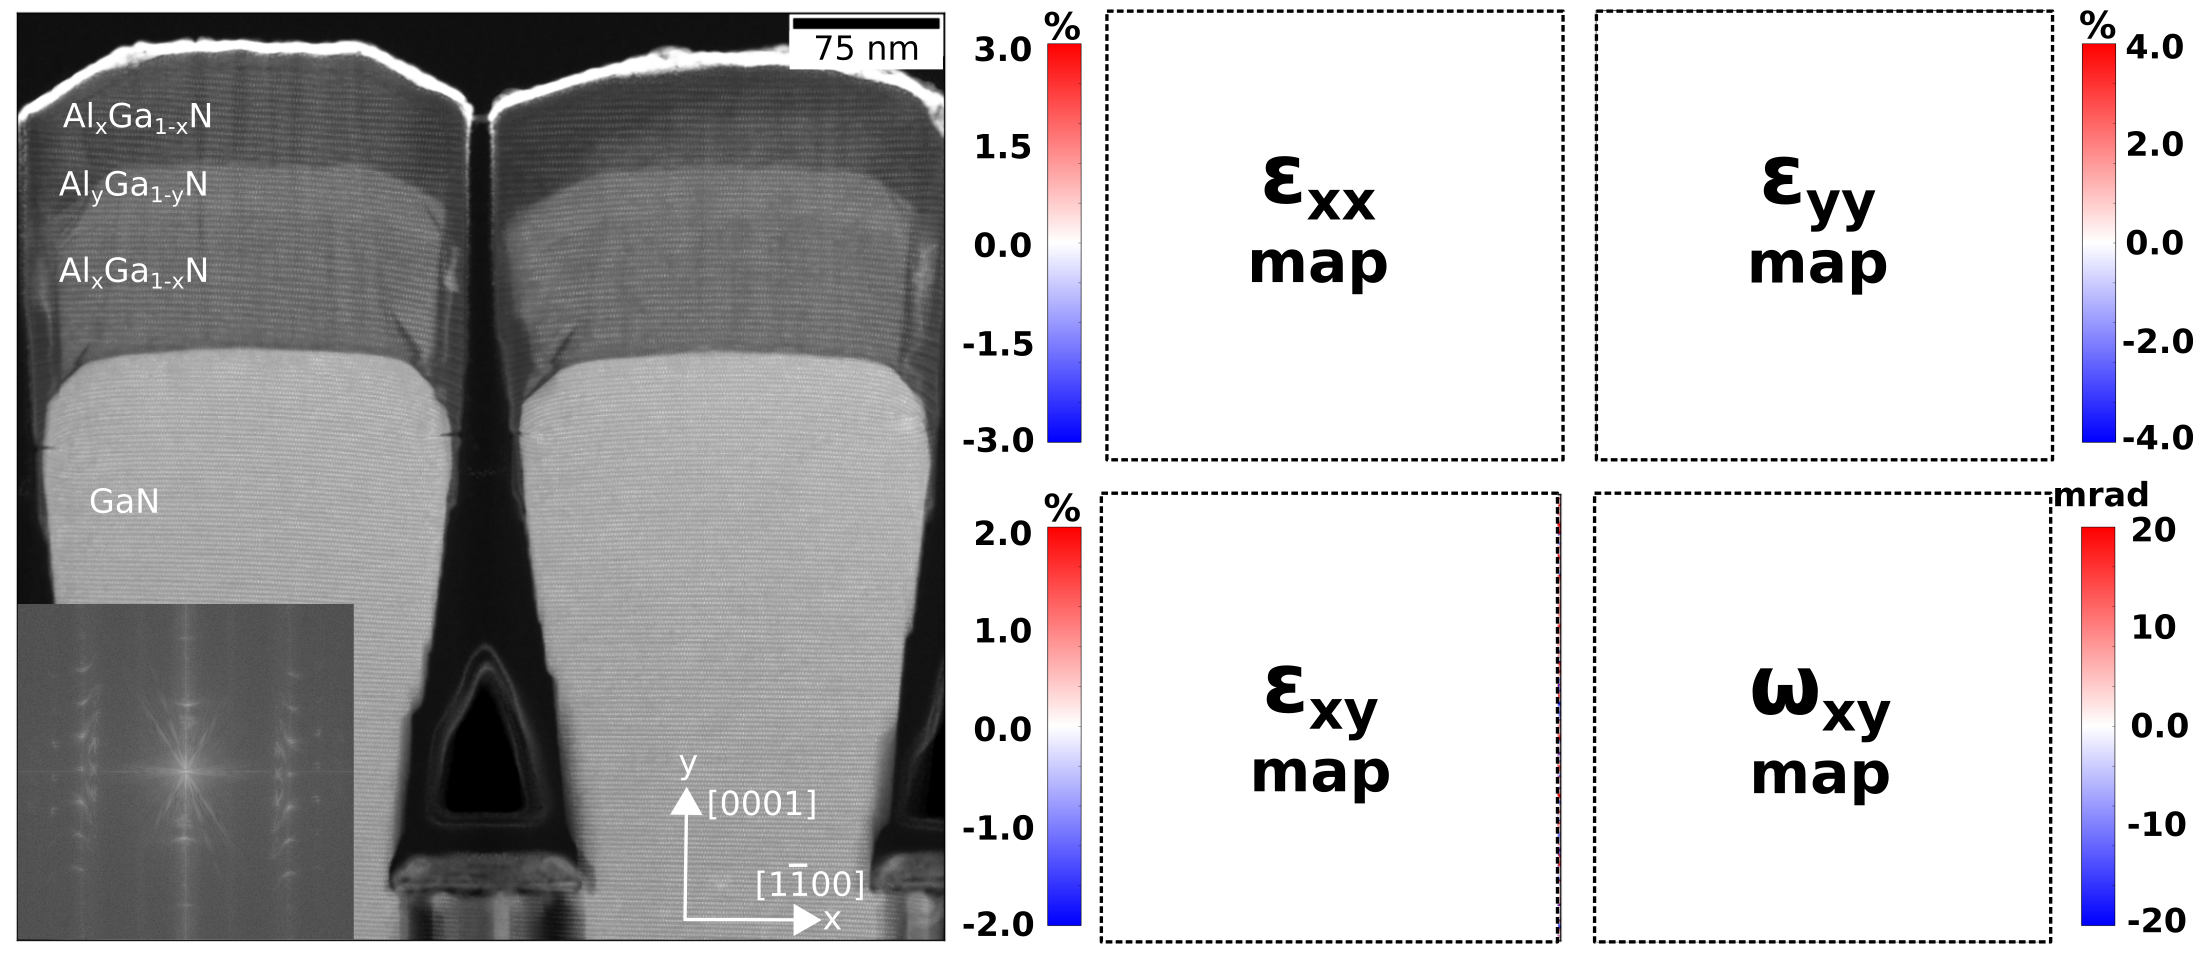
\includegraphics[width=\linewidth]{Figures/STEM_Moire_GPA_objective.png}
\caption[STEM Moir{\'e} GPA objective]{On the left is presented one STEM Moir{\'e} hologram, with its corresponding fast Fourier transform image highlighted in the bottom left corner, acquired on two AlGaN/GaN nanowire Light Emitting Diode (LED) devices. On the right are highlighted the expected relative strain maps, each one corresponding to their respective component of the strain and rotation tensor}
\label{fig:STEM_Moire_GPA_Objective}
\end{figure}

\section{Interest}

As a characterization technique, the STEM Moir{\'e} interferometry method is relatively easy to implement on any modern transmission electron microscope equipped with a scanning module and a probe corrector. The only requirement once the STEM probe is set up, is to define properly the sampling condition of the scanning grid. In comparison, other holography techniques such as Dark-Field Electron Holography (DEFH) \cite{Hytch2008} requires the use of a biprism to bring in interference the diffracted beam issued from two separated areas. In addition, good quality dark-field holograms can only be achieved if the sampled is tilted to respect the "two beam conditions" which is not straight forward. Other diffraction based techniques such as Nano Beam (Precession) Electron Diffraction (NB(P)ED) \cite{Rouviere2013} can also provide large FOV strain maps with similar simplicity however acquiring a diffraction pattern on each pixel of the map is very time consuming. Therefore, STEM Moir{\'e} GPA appears as a very competitive strain characterization technique with respect to current available methods.\par \medskip
On the program side, a characterization technique cannot exist without a dedicated software because the raw data is nearly unusable until converted into quantified strain maps. Therefore, implement a program and make it available to the research and industry community is mandatory in order to expect the strain characterization method to be recognized and applied. Regarding the applicability of the technique, a wide range of user can be expected (from an expert in the field to an analyst performing routine electron microscopy characterization). 

\bibliography{biblio_pbl_stat}
\bibliographystyle{ieeetr}

\end{document}